\chapter{Experiment}
%% Explain the tasks

%%%\section{System setup}
%%%State diagram of plan
%%%\begin{itemize}
%%%\item Find the valve - sensing
%%%\item Move to the valve - close loop on sensing
%%%\item Grab the valve
%%%\item Jump on the valve
%%%\end{itemize}


%%%\section{Task}\label{sec:task}
%%%Turning a valve with whole body (more of a lever)
%%%\begin{itemize}
%%%\item Find the valve - sensing
%%%\item Move to the valve - close loop on sensing
%%%\item Grab the valve
%%%\item Jump on the valve
%%%\end{itemize}

%%%Controllers
%%%\begin{itemize}
%%%\item Walking
%%%\item Balance
%%%\item Complience
%%%\item IK
%%%\item Visual Servoing
%%%\end{itemize}


This section gives examples of the Hubo-Ach system being used on the physical and simulated systems.  Examples include: a walking controller implementation on the physical robot and in simulation; visual servoing while walking using the physical robot; and active damping implementation using the physical robot.


%%\section{Simulator}\label{sec:simulator}
%%	The simulator used for Hubo-Ach is the OpenHubo.
OpenHubo is an open-source kinematic and dynamic simulator for the the Hubo2 and Hubo2+ series robots.
It was developed by the Drexel Autonomous Systems Lab and runs using the open-source robot simulation environment OpenRAVE\cite{diankovThesis}.
Fig.~\ref{fig:openhubbo} shows the OpenHubo shell model and collision model.

\begin{figure}[thpb]
  \centering
      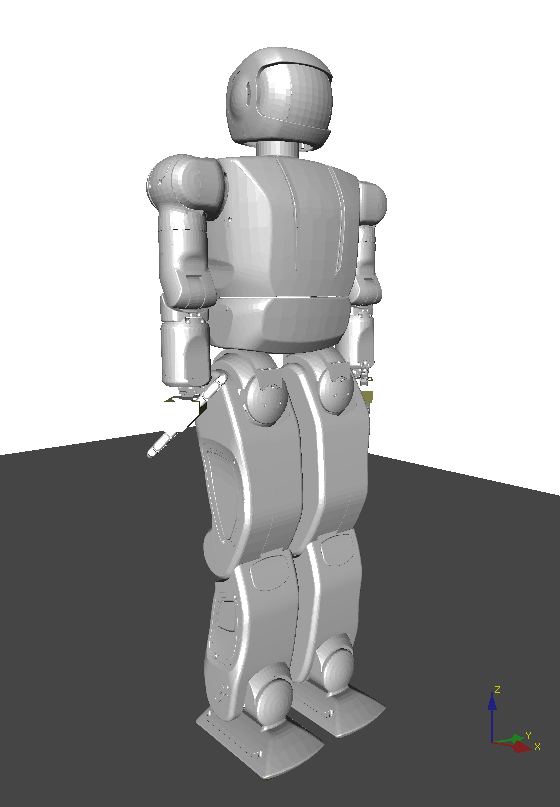
\includegraphics[width=0.4\columnwidth]{./pix/hBody.png}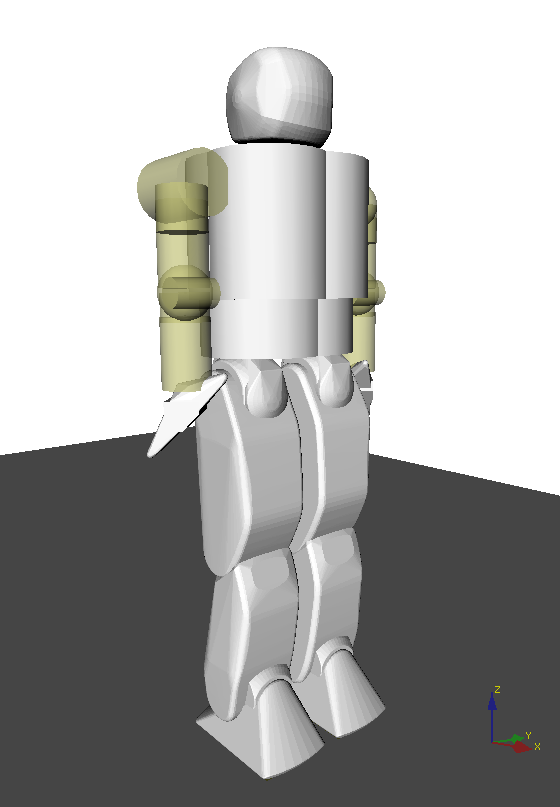
\includegraphics[width=0.4\columnwidth]{./pix/hCol.png}
      
\caption{OpenHubo model of the Hubo2 humanoid robot developed by the Drexel Autonomous Systems Lab and runs using the open-source robot simulation environment OpenRAVE\cite{diankovThesis}.  (Left) Shell Model - High polygon count.  (Right) Collision model - Made with primitives.}
\label{fig:openhubbo}
\end{figure}

The masses and lengths are of the OpenHubo model are all based off of the CAD model.
The shell model includes an external skin based off of the CAD model of the Hubo's shell.
This model is high polygon count and thus tends to require more processing time to detect collisions.
The collision model is constructed out of primitives in order to decrease the complexity of the model and decrease required processing time.
The collision model is a representation of the shell model. 
It does not precisely fit the contours but through experimentation and use has been calibrated to be a good representation of the Hubo's outer shell.

Fig~\ref{fig:openhubosim} shows the diagram of how the OpenHubo simulator is connected to Hubo-Ach.  
No changes to previous controllers are required for them to work with the simulator.
Just as before the desired reference $\theta_d$ being filtered before applied to Hubo via Hubo-Ach.  
$\theta_d$ is sent through a filter that reduces the \textit{jerk} on the actuator then the new reference $\theta_r$ is set on the \textbf{FeedForward} channel, Hubo-Ach reads it then commands Hubo at the rising edge of the next cycle.  
At this point the \textit{to simulator} trigger, $\Gamma_{ts}$, is set high and the OpenHubo simulator reads $\theta_c$.
The simulator waits until Hubo-Ach is ready until it starts its next set of cycles.
The reference is set within OpenHubo and solved with a simulation period of $T_{sim}$.
The simulation period $T_{sim}$ must be an integer deviser of the robot real-time period $T_r$.
In this case

\begin{equation}
T_r=0.005~s
\end{equation}

\begin{equation}
T_{sim} = \frac{T_r}{n}
\end{equation}


Once the simulator has gone through $n$ cycles the current state, $H_{state}$ is placed on the Hubo-Ach \textbf{FeedForward} channel and the ready trigger $\Gamma_{fs}$ is raised.  
Hubo-Ach is waiting for the rising edge of the \textit{from simulator} trigger, $\Gamma_{fs}$, to continue on to the next cycle.

\begin{figure}
\centering

\begin{tikzpicture}[->,>=stealth',shorten >=1pt,auto,node distance=5cm,
  thick,main node/.style={fill=white!20,draw,font=\sffamily\Large\bfseries}]


  \node[main node] (ctrl) {Controller};
  \node[main node] (filter) [right=1.5cm of ctrl] {Filter};
  \node[main node] (hubo-ach) [below=1.0cm of filter] {Hubo-Ach};
  
  \node[main node,font=\small] (hold1) [right=1.5cm of hubo-ach, yshift=0.5cm] {hold};
  \node[main node,font=\small] (hold2) [right=1.5cm of hubo-ach, yshift=-0.5cm] {hold};

  \node[main node] (hubo) [right=1.5cm of hold1, yshift=-0.5cm] {OpenHubo};




%  \path[->, every node/.style={font=\sffamily\small}]
%    (hubo-ach) edge node [above] {$\theta_c$} (hubo);

\draw[->] ([yshift=0.2 cm]hubo-ach.east)  to [out=0,in=-180] node [below] {$\theta_c$} ([yshift=-0.0 cm]hold1.west)  ;
\draw[->] ([yshift=0.0 cm]hold1.east)  to [out=0,in=-180] node [below] {$\theta_c$} ([yshift=0.2 cm]hubo.west)  ;
\draw[-*] ([xshift=1.0 cm]hubo-ach.north)  to [out=60,in=120] node [above] {$\Gamma_{ts}$} ([yshift=-0.05 cm]hold1.north)  ;



\draw[->] ([yshift=0.0 cm]hold2.west)  to [out=180,in=0] node [below] {$H_{state}$} ([yshift=-0.2 cm]hubo-ach.east)  ;
\draw[->] ([yshift=-0.2 cm]hubo.west)  to [out=180,in=0] node [below right] {$H_{state}$} ([yshift=0.0 cm]hold2.east)  ;
\draw[-*] ([xshift=0.0 cm]hubo.south)  to [out=-120,in=-60] node [above] {$\Gamma_{fs}$} ([yshift=0.05 cm]hold2.south)  ;

\draw[->] ([yshift=-0.0 cm]hubo-ach.west)  to [out=180,in=-90] node [below left] {$H_{state}$} ([yshift=0.0 cm]ctrl.south)  ;



%\draw[->] ([yshift=-0.2 cm]hubo.west)  -- node [below] {$H_{state}$} ([yshift=-0.2 cm]hubo-ach.east)  ;
%\draw[->] ([yshift=-0.0 cm]hubo.south)  to [out=-120,in=-60] node [below] {$\Gamma_{fs}$} ([yshift=-0.0 cm]hubo-ach.south)  ;



  \path[->,every node/.style={font=\sffamily\small}]
    (ctrl) edge node [above] {$\theta_d$} (filter);

 \draw[->] ([xshift=-0.5 cm]filter.south)  -- node [left] {$\theta_r$} ([xshift=-0.5 cm]hubo-ach.north)  ;
 \draw[->] ([xshift=0.5 cm]hubo-ach.north) -- node [left] {$\theta_a$} ([xshift=0.5 cm]filter.south)  ;


\end{tikzpicture}
\caption{Desired reference $\theta_d$ being filtered before applied to Hubo via Hubo-Ach.  $\theta_d$ is sent through a filter that reduces the \textit{jerk} on the actuator then the new reference $\theta_r$ is set on the \textbf{FeedForward} channel, Hubo-Ach reads it then commands Hubo at the rising edge of the next cycle.}
\label{fig:hubo-ach-feedforwardFilter}
\end{figure}




The external controllers do not know weather Hubo-Ach is running in \textit{simulation} or \textit{real-time} mode.  
In order to ensure a Hubo-Ach controller stays what ever timing method is being used the controller can do any of the following:

\begin{itemize}
\item Wait for the $\Gamma_{fs}$ trigger
\item Wait for a new $H_P{state}$ to be updated
\item Watch the time listed within $H_{state}$
\end{itemize}

If the given task does not require physics or feedback from $H_{state}$ then you can run in \textit{no physics} mode.
\textit{No physics} mode only gives collisions, joint angles and ideal feedback from the sensors.
In addition \textit{no physics} is capable of running much faster then real-time if needed.



\begin{table}
\centering
\caption{OpenHubo simulator sim-time and real-time comparison chart.  Shows the maximum percent real-time the OpenHubo simulator is capable of preforming at where 100\% is real-time.  All tests were preformed on an Intel i7 running at 2.8Ghz with 18Gb of RAM.}
\begin{tabular}{| l || c | c |}
\hline
Mode               & Timing                & Maximum Percent Real-Time (\%) \\
\hline
\hline
Physics            & Sim-Time              & 37\%   \\
\hline
No Physics         & Real-Time or Sim-Time & 362\%  \\
\hline
\end{tabular}\label{table:simtime}
\end{table}


Fig.~\ref{fig:huboOpenHuboWalking} shows the capability of Hubo-Ach to run in both sim-time and real-time modes.  
This is the same statically stable trajectory as seen in Section~\ref{sec:WalkingPatternGeneration}


\begin{figure}[thpb]
  \centering
      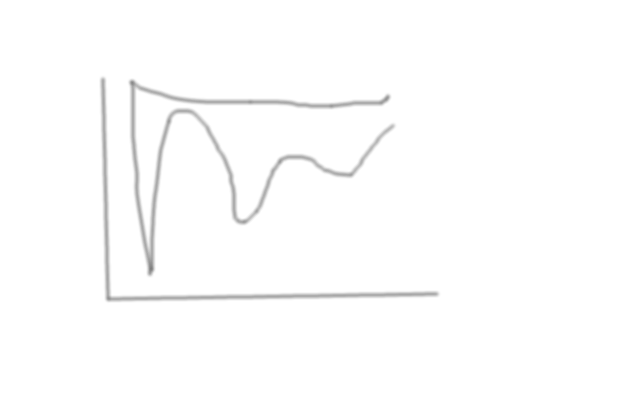
\includegraphics[width=0.69\columnwidth]{./pix/tmp.png}
      
\includegraphics[width=0.3\columnwidth]{./qrcode/qrcode-hubo-openhubo-walking.png}\\
      Video: http://danlofaro.com/phd/walking/\#WalkingHuboAndOpenHubo
\caption{Hubo and OpenHubo walking using Hubo-Ach in Real-Time and Sim-Time Respectively}
\label{fig:huboOpenHuboWalking}
\end{figure}


	%% show balance in simulator too




\section{Walking}\label{sec:walking:example}
	%% Sim walking too
	This section shows examples of how Hubo-Ach was used for stable walking.
Examples are given using:
\begin{itemize}
\item Hubo2+ (Physical Robot)
\item OpenHubo (Simulator)
\item RobotSim Hubo (Simulator)
\end{itemize}

section~\ref{sec:WalkingPatternGeneration} shows how the open-loop walking trajectory is created.

Section~\ref{sec:OpenHuboWalking} shows how the open loop walking trajectory is run in sim-time on OpenHubo using Hubo-Ach.
Section~\ref{sec:RobotSimWalking} shows how the open loop walking trajectory is run in sim-time on RobotSim using Hubo-Ach.
Section~\ref{sec:HuboWalking} shows the same walking trajectory running on the real Hubo hardware in real-time using Hubo-Ach.
It also shows the difference between running in sim-time and real-time.
Section~\ref{sec:dynamicWalking} shows the result of a five day \textit{hack-a-thon} using Hubo-Ach to add dynamic walking capability.





%% ---------------- Walking Pattern Generation ------------------------
\subsection{Walking Pattern Generation}\label{sec:WalkingPatternGeneration}
The walking pattern demonstrated in this section is generated based on the work of Park et. al.\cite{4115633}
A walking pattern is the way in which a legged robot, in this case two legged, moves its joints to create a walking gate while maintaining stability.
The walking pattern consists of two major phases:
\begin{itemize}
\item Single Support Phase (SSP)
\item Double Support Phase (DSP)
\end{itemize}

\noindent \textbf{Single support phase} is when one foot is on the ground.
This phase is when one leg moves from one stepping position to the other.
The ZMP must remain above the planted foot to guarantee stability.\\

\noindent \textbf{Double support phase} is when both feet are planted on the ground.  
When in this phase the ZMP moves from above one foot to the other along the stable area as seen in Fig.~\ref{fig:zmp}.




\begin{figure}[t]
  \centering
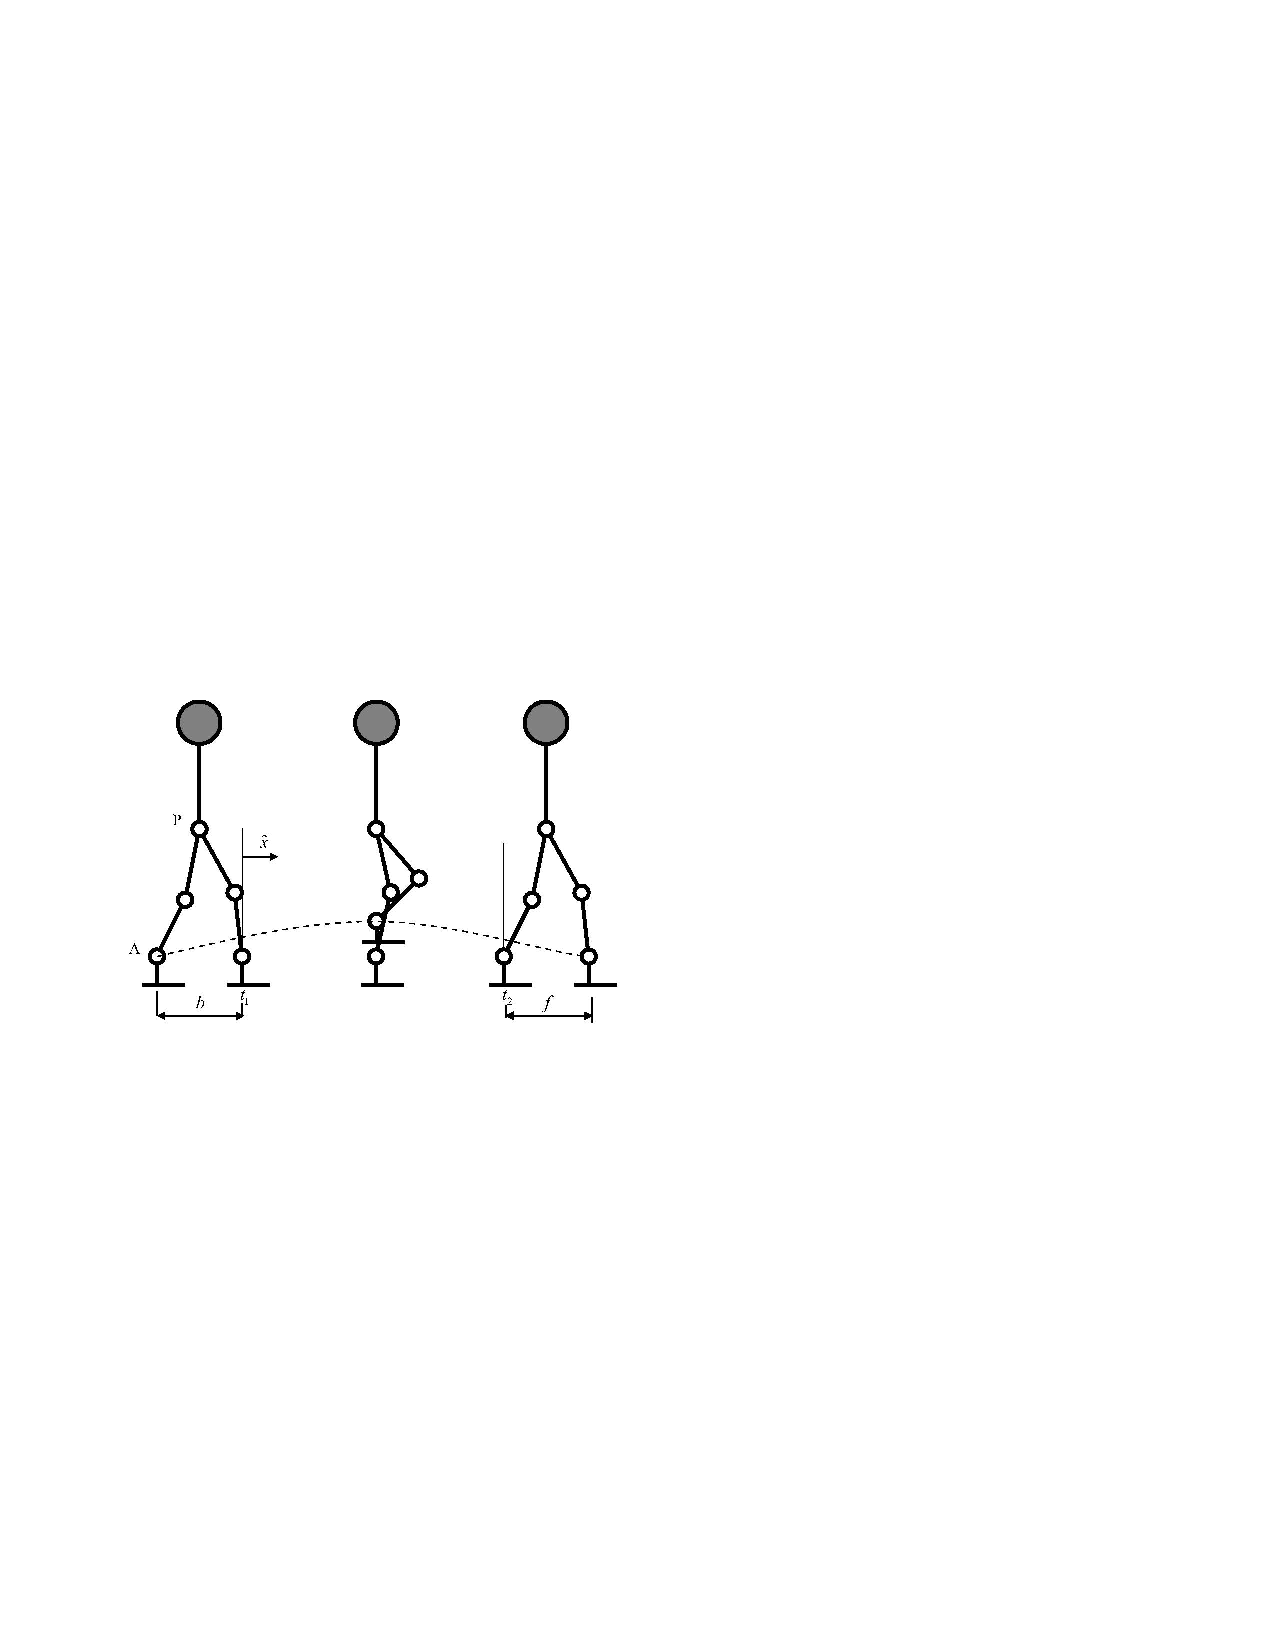
\includegraphics[width=0.5\columnwidth]{./examples/pix/huboZMPx.pdf}
  \caption{Hubo model diagram for ZMP walking in the $x$ direction (side view).  $b$ and $f$ are the step lengths for the left and the right foot.  $A$ defines the ankle.  $t_1$ is the time of the starting of the step, $t_2$ defines the landing of the stepping foot.  $P$ defines the hip location.  $\widetilde{x}$ defines the walking velocity.  The middle diagram depicts the SSP and the left and right diagrams show the DSP.}
  \label{fig:huboZMPx}
\end{figure}

Fig~\ref{fig:huboZMPx} and \ref{fig:huboZMPy} shows the walking pattern phases on a Hubo model in the $x$ and $y$ direction respectively.
In these figures $A_R$ and $A_L$ defines the left and right ankles respectively.  
$t_1$ is the time of the starting of the step, $t_2$ defines the landing of the stepping foot.  
$t_0$ defines time when the stepping foot is at peak step height.  
$P$ defines the hip location.  
$\widetilde{x}$ defines the walking velocity.
$\widetilde{y}$ defines the body sway velocity.  
The middle diagram depicts the SSP and the left and right diagrams show the DSP.



\begin{figure}[t]
  \centering
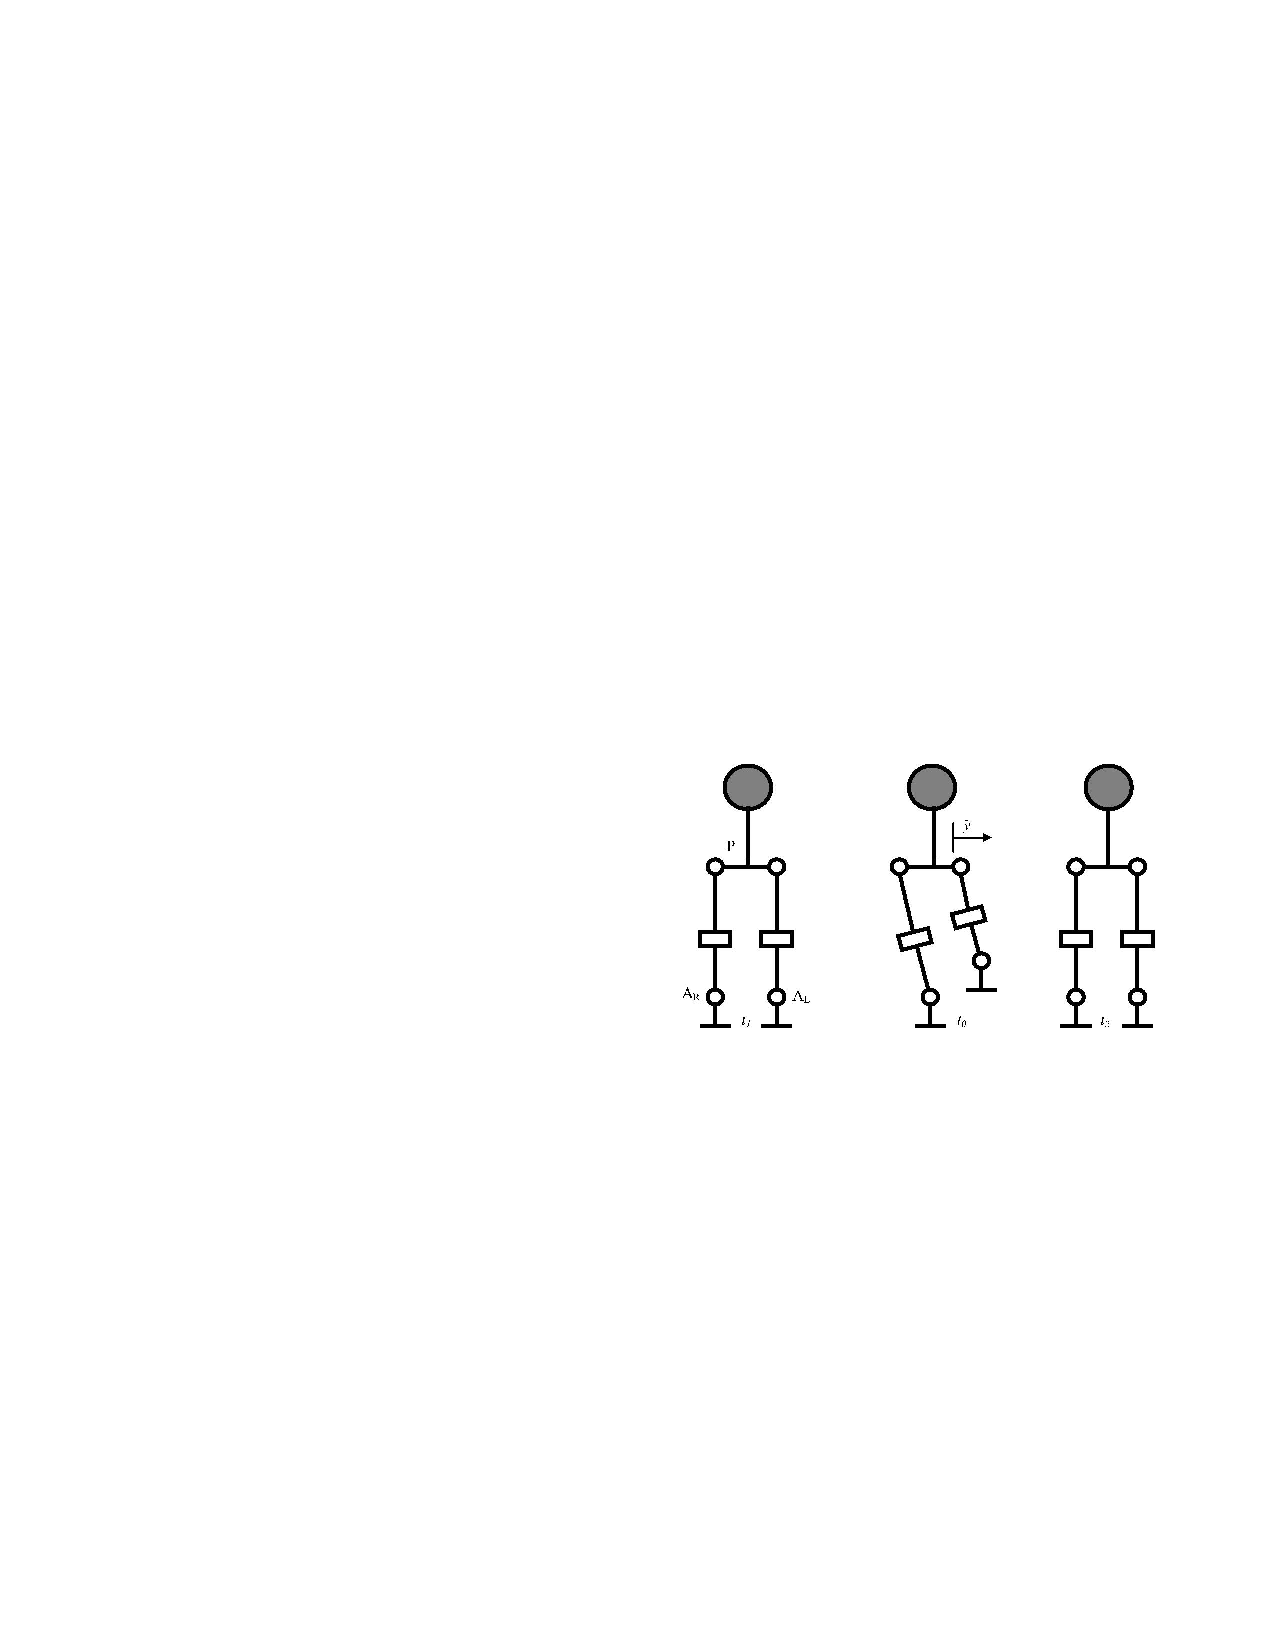
\includegraphics[width=0.7\columnwidth]{./examples/pix/huboZMPy.pdf}
  \caption{Hubo model diagram for ZMP walking in the $y$ direction (front view).  $A_R$ and $A_L$ defines the left and right ankles respectively.  $t_1$ is the time of the starting of the step, $t_2$ defines the landing of the stepping foot.  $t_0$ defines time when the stepping foot is at peak step height.  $P$ defines the hip location.  $\widetilde{y}$ defines the body sway velocity.  The middle diagram depicts the SSP and the left and right diagrams show the DSP.}
  \label{fig:huboZMPy}
\end{figure}


The walking patterns are generated creating a joint space trajectory with a period $T$ of $0.005~sec$.
The patterns keep the ZMP criteria described in Section~\ref{sec:zmp}.
These walking patterns are used to test the simulated robots and the physical robots.
Fig.~\ref{fig:huboZMPjointSpace} shows the joint space walking pattern verses time.

\begin{figure}[t]
  \centering
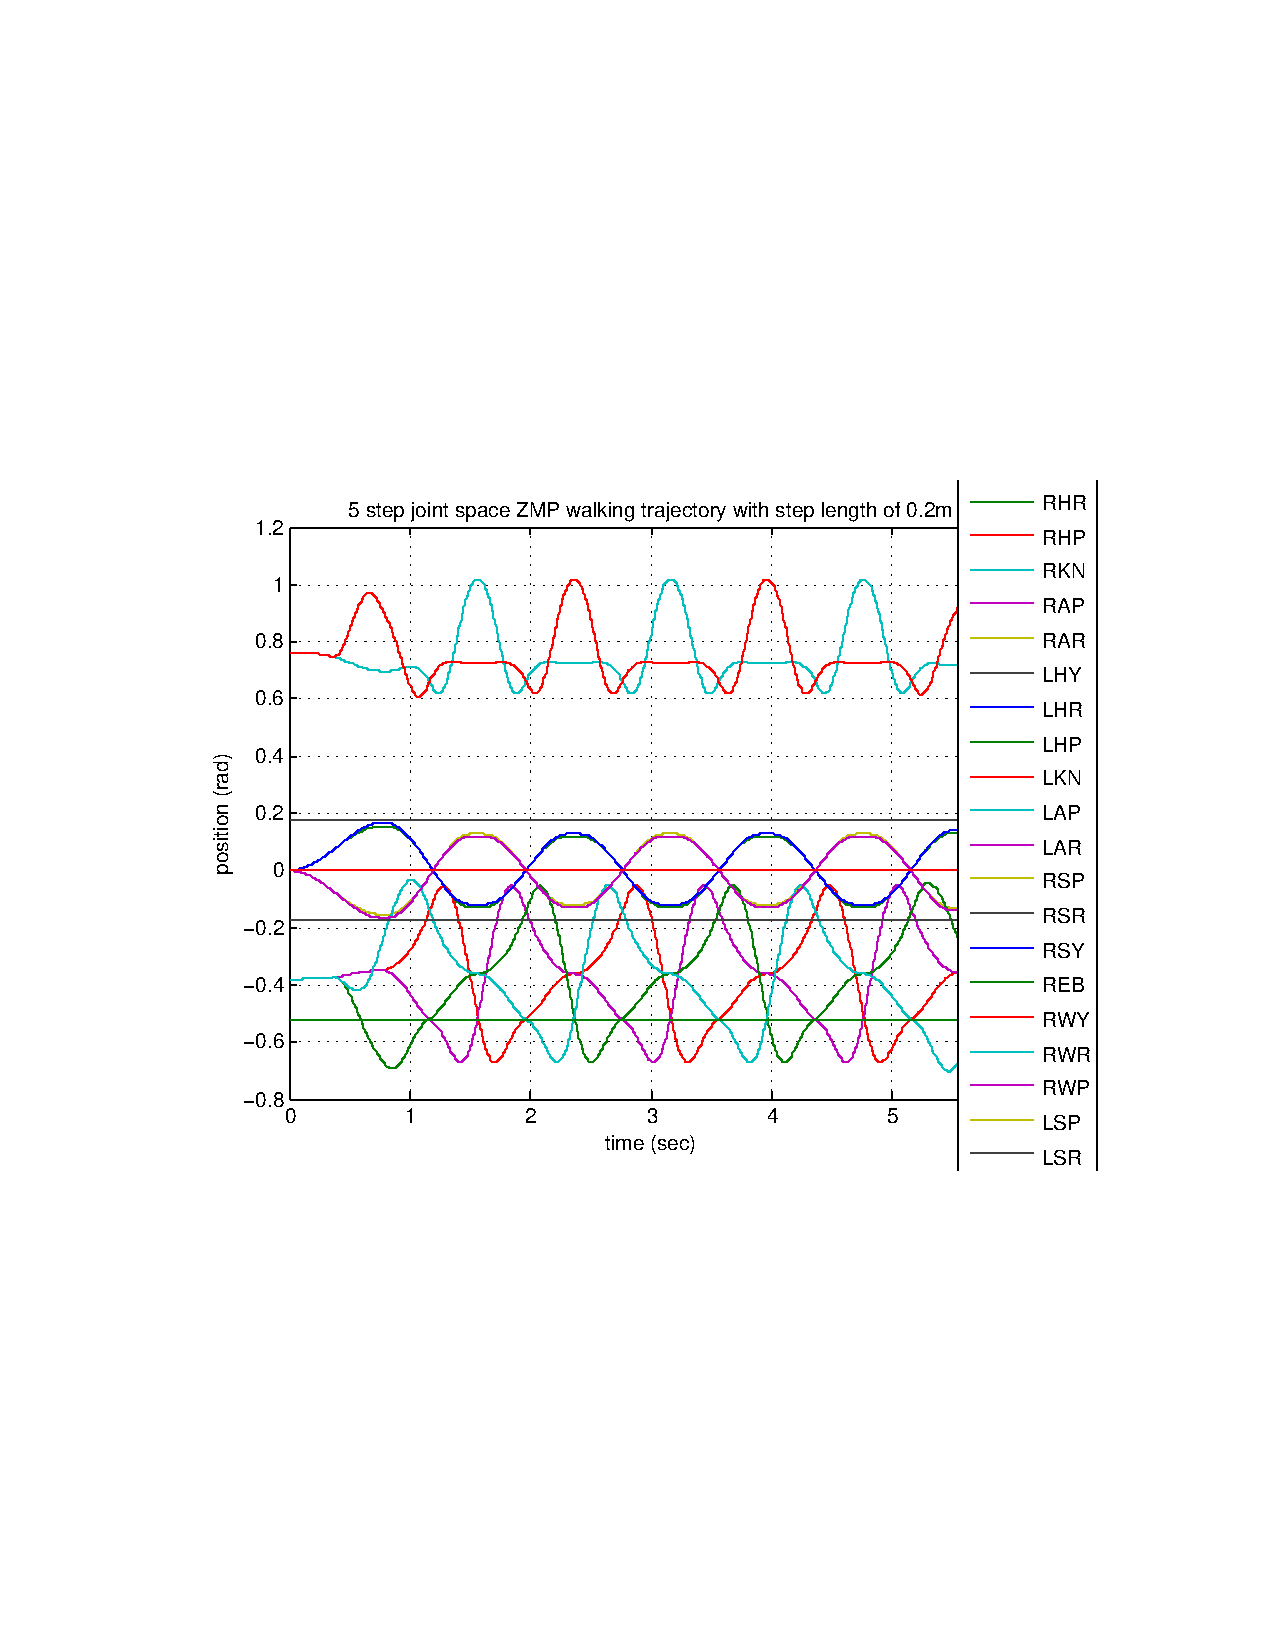
\includegraphics[width=0.8\columnwidth]{./pix/walk5step.pdf}
  \caption{Joint space walking pattern.  The trajectory sampling period $T$ is $0.005~sec$.  Forward step length is $0.2~m$, sway velocity $\widetilde{y}$ is $0.062~\frac{m}{sec}$, and step period is $0.8~sec$.}
  \label{fig:huboZMPjointSpace}
\end{figure}





%% ---------------- OpenHubo Walking ------------------------
\subsection{Walking Using OpenHubo Simulator and Hubo-Ach}\label{sec:OpenHuboWalking}

The walking pattern that was generated in Section~\ref{sec:WalkingPatternGeneration} was then applied to the OpenHubo system described in Section~\ref{sec:simulator} via the Hubo-Ach controller.
The walking pattern was applied in sim-time with a period $T_{sim}$ of $0.005~sec$.
The block diagram of the system using OpenHubo in sim-time for a walking trajectory is shown in Fig.~\ref{fig:openhubosimWalking}.

\begin{figure}
\centering

\begin{tikzpicture}[->,>=stealth',shorten >=1pt,auto,node distance=5cm,
  thick,main node/.style={fill=white!20,draw,font=\sffamily\Large\bfseries}]


  \node[main node] (ctrl) [text width=3cm] {Walking Pattern};
 
  \node[main node] (hubo-ach) [right=1.5cm of ctrl] {Hubo-Ach};
  
  \node[main node,font=\small] (hold1) [right=1.5cm of hubo-ach, yshift=0.5cm] {hold};
  \node[main node,font=\small] (hold2) [right=1.5cm of hubo-ach, yshift=-0.5cm] {hold};
  \node[main node,font=\small] (hold3) [below=0cm of ctrl, yshift=0.0cm] {hold};


  \node[main node] (hubo) [right=1.5cm of hold1, yshift=-0.5cm] {OpenHubo};




%  \path[->, every node/.style={font=\sffamily\small}]
%    (hubo-ach) edge node [above] {$\theta_c$} (hubo);

\draw[->] ([yshift=0.2 cm]hubo-ach.east)  to [out=0,in=-180] node [below] {$\theta_c$} ([yshift=-0.0 cm]hold1.west)  ;
\draw[->] ([yshift=0.0 cm]hold1.east)  to [out=0,in=-180] node [below] {$\theta_c$} ([yshift=0.2 cm]hubo.west)  ;
\draw[-*] ([xshift=1.0 cm]hubo-ach.north)  to [out=60,in=120] node [above] {$\Gamma_{ts}$} ([yshift=-0.05 cm]hold1.north)  ;
%\draw[-*] ([xshift=-0.02 cm]hubo-ach.north)  to [out=120,in=60] node [above] {$\Gamma_{ts}$} ([yshift=-0.05 cm]hold3.north)  ;



\draw[->] ([yshift=0.0 cm]hold2.west)  to [out=180,in=0] node [below] {$H_{state}$} ([yshift=-0.2 cm]hubo-ach.east)  ;
\draw[->] ([yshift=-0.2 cm]hubo.west)  to [out=180,in=0] node [below right] {$H_{state}$} ([yshift=0.0 cm]hold2.east)  ;
\draw[-*] ([xshift=-0.02 cm]hubo.south)  to [out=-120,in=-60] node [above] {$\Gamma_{fs}$} ([yshift=0.05 cm]hold2.south)  ;
\draw[-*] ([xshift=0.02 cm]hubo.south)  to [out=-115,in=-55] node [above] {$\Gamma_{fs}$} ([yshift=0.05 cm]hold3.south)  ;

\draw[-*] (hold3.north)  to [out=90,in=-90] node [above] {}(ctrl.south)  ;

%\draw[->] ([yshift=-0.0 cm]hubo-ach.west)  to [out=180,in=-90] node [below left] {$H_{state}$} ([yshift=0.0 cm]ctrl.south)  ;



%\draw[->] ([yshift=-0.2 cm]hubo.west)  -- node [below] {$H_{state}$} ([yshift=-0.2 cm]hubo-ach.east)  ;
%\draw[->] ([yshift=-0.0 cm]hubo.south)  to [out=-120,in=-60] node [below] {$\Gamma_{fs}$} ([yshift=-0.0 cm]hubo-ach.south)  ;



  \path[->,every node/.style={font=\sffamily\small}]
    (ctrl) edge node [above] {$\theta_r$} (hubo-ach);



\end{tikzpicture}
\caption{Diagram of how the OpenHubo simulator is connected to Hubo-Ach and is used to run a walking trajectory.  
The walking pattern generator ensures proper constraints on the velocity, acceleration and jerk and thus the filter seen in Fig.~\ref{fig:openhubosim} is not desired.  
$\theta_r$ is set directly on the \textbf{FeedForward} channel thus each joint will have the response as seen in Fig.~\ref{fig:singleJointStep} for each commanded reference command at each time step.
Hubo-Ach reads the \textbf{FeedForward} channel and commands Hubo at the rising edge of the next cycle.  
At this point $\Gamma_{ts}$ is set high and the OpenHubo simulator reads $\theta_c$.  
The reference is set within OpenHubo and solved with a simulation period of $T_{sim}$.  
Once The state, $H_{state}$ has been determined it is placed on the Hubo-Ach \textbf{FeedForward} channel and the ready trigger $\Gamma_{fs}$ is raised.  
Hubo-Ach is waiting for the rising edge of $\Gamma_{fs}$ to continue on to the next cycle.  
In order to keep with the sim-time the \textit{Walking Pattern} also waits for the rising edge of $\Gamma_{fs}$ to put the next desired reference on the \textbf{FeedForward} channel. }
\label{fig:openhubosimWalking}
\end{figure}



In Fig.~\ref{fig:openhubosimWalking} the OpenHubo simulator is connected to Hubo-Ach and is used to run the walking trajectory.  
The walking pattern generator ensures proper constraints on the velocity, acceleration and jerk and thus the filter seen in Fig.~\ref{fig:openhubosim} is not desired.  
$\theta_r$ is set directly on the \textbf{FeedForward} channel thus each joint will have the response as seen in Fig.~\ref{fig:singleJointStep} for each commanded reference command at each time step.
Hubo-Ach reads the \textbf{FeedForward} channel and commands Hubo at the rising edge of the next cycle.  
At this point $\Gamma_{ts}$ is set high and the OpenHubo simulator reads $\theta_c$.  
The reference is set within OpenHubo and solved with a simulation period of $T_{sim}$.  
Once The state, $H_{state}$ has been determined it is placed on the Hubo-Ach \textbf{FeedForward} channel and the ready trigger $\Gamma_{fs}$ is raised.  
Hubo-Ach is waiting for the rising edge of $\Gamma_{fs}$ to continue on to the next cycle.  
In order to keep with the sim-time the \textit{Walking Pattern} also waits for the rising edge of $\Gamma_{fs}$ to put the next desired reference on the \textbf{FeedForward} channel.
Fig.~\ref{fig:openHuboWalkingVideo} shows the Virtual Hubo successfully ZMP walking using OpenHubo and Hubo-Ach.

\begin{figure}[thpb]
  \centering
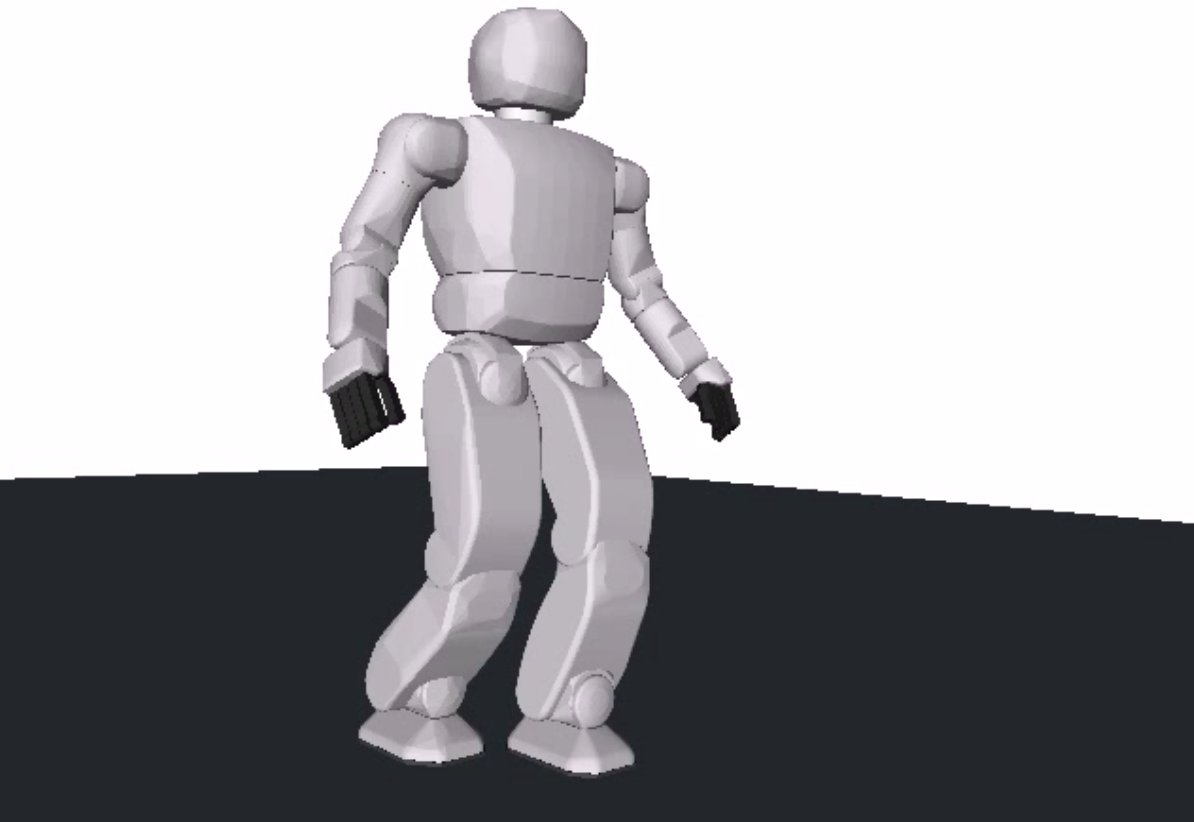
\includegraphics[width=0.6\columnwidth]{./examples/pix/openhubo-walking.png}

\includegraphics[width=0.3\columnwidth]{./qrcode/qrcode-openhubo-walking.png}\\
      Video: http://danlofaro.com/phd/walking/\#WalkingOpenHubo
  \caption{Virtual Hubo in OpenHubo preforming ZMP walking using Hubo-Ach in sim-time based on the walking pattern generated in Section~\ref{sec:WalkingPatternGeneration}}
  \label{fig:openHuboWalkingVideo}
\end{figure}




%% ---------------- OpenHubo Walking ------------------------
\subsection{Walking Using RobotSim and Hubo-Ach}\label{sec:RobotSimWalking}
\begin{figure}[thpb]
  \centering
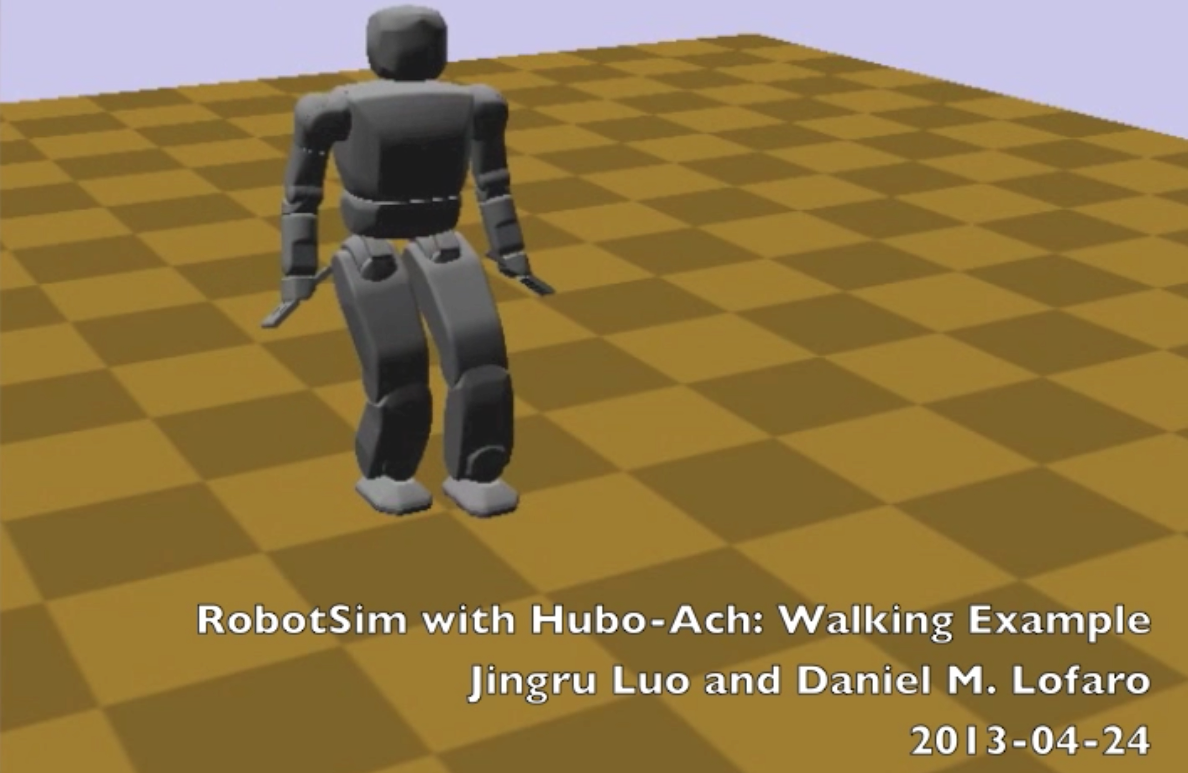
\includegraphics[width=0.6\columnwidth]{./examples/pix/robotsim-walking.png}

\includegraphics[width=0.3\columnwidth]{./qrcode/qrcode-robotsim-walking.png}\\
      Video: http://danlofaro.com/phd/walking/\#WalkingRobotSim
  \caption{Virtual Hubo in RobotSim preforming ZMP walking using Hubo-Ach in sim-time based on the walking pattern generated in Section~\ref{sec:WalkingPatternGeneration}}
  \label{fig:robotSimWalkingVideo}
\end{figure}

The walking pattern that was generated in Section~\ref{sec:WalkingPatternGeneration} was then applied to the RobotSim dynamic simulator via the Hubo-Ach controller.
RobotSim was developed by Professor Kris Hauser from Indiana University.
The simulator was integrated into Hubo-Ach on April 24$^{th}$, 2013 during a 12 hour \textit{Hack-A-Thon} at Worchester Polytechnic Institute by Daniel M. Lofaro, Jingru Luo and Professor Kris Hauser\cite{wpiHackathon}.
The walking pattern was applied in sim-time with a period $T_{sim}$ of $0.005~sec$.
The block diagram of the system using RobotSim in sim-time for a walking trajectory is shown in Fig.~\ref{fig:RobotSimWalking}.

\begin{figure}
\centering

\begin{tikzpicture}[->,>=stealth',shorten >=1pt,auto,node distance=5cm,
  thick,main node/.style={fill=white!20,draw,font=\sffamily\Large\bfseries}]


  \node[main node] (ctrl) [text width=3cm] {Walking Pattern};
 
  \node[main node] (hubo-ach) [right=1.5cm of ctrl] {Hubo-Ach};
  
  \node[main node,font=\small] (hold1) [right=1.5cm of hubo-ach, yshift=0.5cm] {hold};
  \node[main node,font=\small] (hold2) [right=1.5cm of hubo-ach, yshift=-0.5cm] {hold};
  \node[main node,font=\small] (hold3) [below=0cm of ctrl, yshift=0.0cm] {hold};


  \node[main node] (hubo) [right=1.5cm of hold1, yshift=-0.5cm] {OpenHubo};




%  \path[->, every node/.style={font=\sffamily\small}]
%    (hubo-ach) edge node [above] {$\theta_c$} (hubo);

\draw[->] ([yshift=0.2 cm]hubo-ach.east)  to [out=0,in=-180] node [below] {$\theta_c$} ([yshift=-0.0 cm]hold1.west)  ;
\draw[->] ([yshift=0.0 cm]hold1.east)  to [out=0,in=-180] node [below] {$\theta_c$} ([yshift=0.2 cm]hubo.west)  ;
\draw[-*] ([xshift=1.0 cm]hubo-ach.north)  to [out=60,in=120] node [above] {$\Gamma_{ts}$} ([yshift=-0.05 cm]hold1.north)  ;
%\draw[-*] ([xshift=-0.02 cm]hubo-ach.north)  to [out=120,in=60] node [above] {$\Gamma_{ts}$} ([yshift=-0.05 cm]hold3.north)  ;



\draw[->] ([yshift=0.0 cm]hold2.west)  to [out=180,in=0] node [below] {$H_{state}$} ([yshift=-0.2 cm]hubo-ach.east)  ;
\draw[->] ([yshift=-0.2 cm]hubo.west)  to [out=180,in=0] node [below right] {$H_{state}$} ([yshift=0.0 cm]hold2.east)  ;
\draw[-*] ([xshift=-0.02 cm]hubo.south)  to [out=-120,in=-60] node [above] {$\Gamma_{fs}$} ([yshift=0.05 cm]hold2.south)  ;
\draw[-*] ([xshift=0.02 cm]hubo.south)  to [out=-115,in=-55] node [above] {$\Gamma_{fs}$} ([yshift=0.05 cm]hold3.south)  ;

\draw[-*] (hold3.north)  to [out=90,in=-90] node [above] {}(ctrl.south)  ;

%\draw[->] ([yshift=-0.0 cm]hubo-ach.west)  to [out=180,in=-90] node [below left] {$H_{state}$} ([yshift=0.0 cm]ctrl.south)  ;



%\draw[->] ([yshift=-0.2 cm]hubo.west)  -- node [below] {$H_{state}$} ([yshift=-0.2 cm]hubo-ach.east)  ;
%\draw[->] ([yshift=-0.0 cm]hubo.south)  to [out=-120,in=-60] node [below] {$\Gamma_{fs}$} ([yshift=-0.0 cm]hubo-ach.south)  ;



  \path[->,every node/.style={font=\sffamily\small}]
    (ctrl) edge node [above] {$\theta_r$} (hubo-ach);



\end{tikzpicture}
\caption{Diagram of how the OpenHubo simulator is connected to Hubo-Ach and is used to run a walking trajectory.  
The walking pattern generator ensures proper constraints on the velocity, acceleration and jerk and thus the filter seen in Fig.~\ref{fig:openhubosim} is not desired.  
$\theta_r$ is set directly on the \textbf{FeedForward} channel thus each joint will have the response as seen in Fig.~\ref{fig:singleJointStep} for each commanded reference command at each time step.
Hubo-Ach reads the \textbf{FeedForward} channel and commands Hubo at the rising edge of the next cycle.  
At this point $\Gamma_{ts}$ is set high and the OpenHubo simulator reads $\theta_c$.  
The reference is set within OpenHubo and solved with a simulation period of $T_{sim}$.  
Once The state, $H_{state}$ has been determined it is placed on the Hubo-Ach \textbf{FeedForward} channel and the ready trigger $\Gamma_{fs}$ is raised.  
Hubo-Ach is waiting for the rising edge of $\Gamma_{fs}$ to continue on to the next cycle.  
In order to keep with the sim-time the \textit{Walking Pattern} also waits for the rising edge of $\Gamma_{fs}$ to put the next desired reference on the \textbf{FeedForward} channel. }
\label{fig:openhubosimWalking}
\end{figure}



In Fig.~\ref{fig:RobotSimWalking} the RobotSim simulator is connected to Hubo-Ach and is used to run the walking trajectory.  
The walking pattern generator ensures proper constraints on the velocity, acceleration and jerk and thus the filter seen in Fig.~\ref{fig:openhubosim} is not desired.  
$\theta_r$ is set directly on the \textbf{FeedForward} channel thus each joint will have the response as seen in Fig.~\ref{fig:singleJointStep} for each commanded reference command at each time step.
Hubo-Ach reads the \textbf{FeedForward} channel and commands Hubo at the rising edge of the next cycle.  
At this point $\Gamma_{ts}$ is set high and the RobotSim simulator reads $\theta_c$.  
The reference is set within RobotSim and solved with a simulation period of $T_{sim}$.  
Once The state, $H_{state}$ has been determined it is placed on the Hubo-Ach \textbf{FeedForward} channel and the ready trigger $\Gamma_{fs}$ is raised.  
Hubo-Ach is waiting for the rising edge of $\Gamma_{fs}$ to continue on to the next cycle.  
In order to keep with the sim-time the \textit{Walking Pattern} also waits for the rising edge of $\Gamma_{fs}$ to put the next desired reference on the \textbf{FeedForward} channel.
Fig.~\ref{fig:robotSimWalkingVideo} shows the Virtual Hubo successfully ZMP walking using RobotSim and Hubo-Ach.

\begin{figure}
\centering

\begin{tikzpicture}[->,>=stealth',shorten >=1pt,auto,node distance=5cm,
  thick,main node/.style={fill=white!20,draw,font=\sffamily\Large\bfseries}]


  \node[main node] (ctrl) [text width=3cm] {Walking Pattern};
 
  \node[main node] (hubo-ach) [right=1.5cm of ctrl] {Hubo-Ach};
  
  \node[main node,font=\small] (hold1) [right=1.5cm of hubo-ach, yshift=0.5cm] {hold};
  \node[main node,font=\small] (hold2) [right=1.5cm of hubo-ach, yshift=-0.5cm] {hold};
  \node[main node,font=\small] (hold3) [below=0.0cm of ctrl, yshift=0.0cm] {hold};


  \node[main node] (hubo) [right=1.5cm of hold1, yshift=-0.5cm] {RobotSim};




%  \path[->, every node/.style={font=\sffamily\small}]
%    (hubo-ach) edge node [above] {$\theta_c$} (hubo);

\draw[->] ([yshift=0.2 cm]hubo-ach.east)  to [out=0,in=-180] node [below] {$\theta_c$} ([yshift=-0.0 cm]hold1.west)  ;
\draw[->] ([yshift=0.0 cm]hold1.east)  to [out=0,in=-180] node [below] {$\theta_c$} ([yshift=0.2 cm]hubo.west)  ;
\draw[-*] ([xshift=1.0 cm]hubo-ach.north)  to [out=60,in=120] node [above] {$\Gamma_{ts}$} ([yshift=-0.05 cm]hold1.north)  ;
%\draw[-*] ([xshift=-0.02 cm]hubo-ach.north)  to [out=120,in=60] node [above] {$\Gamma_{ts}$} ([yshift=-0.05 cm]hold3.north)  ;



\draw[->] ([yshift=0.0 cm]hold2.west)  to [out=180,in=0] node [below] {$H_{state}$} ([yshift=-0.2 cm]hubo-ach.east)  ;
\draw[->] ([yshift=-0.2 cm]hubo.west)  to [out=180,in=0] node [below right] {$H_{state}$} ([yshift=0.0 cm]hold2.east)  ;
\draw[-*] ([xshift=-0.02 cm]hubo.south)  to [out=-120,in=-60] node [above] {$\Gamma_{fs}$} ([yshift=0.05 cm]hold2.south)  ;
\draw[-*] ([xshift=0.02 cm]hubo.south)  to [out=-115,in=-55] node [above] {$\Gamma_{fs}$} ([yshift=0.05 cm]hold3.south)  ;

\draw[-*] (hold3.north)  to [out=90,in=-90] node [above] {}(ctrl.south)  ;

%\draw[->] ([yshift=-0.0 cm]hubo-ach.west)  to [out=180,in=-90] node [below left] {$H_{state}$} ([yshift=0.0 cm]ctrl.south)  ;



%\draw[->] ([yshift=-0.2 cm]hubo.west)  -- node [below] {$H_{state}$} ([yshift=-0.2 cm]hubo-ach.east)  ;
%\draw[->] ([yshift=-0.0 cm]hubo.south)  to [out=-120,in=-60] node [below] {$\Gamma_{fs}$} ([yshift=-0.0 cm]hubo-ach.south)  ;



  \path[->,every node/.style={font=\sffamily\small}]
    (ctrl) edge node [above] {$\theta_r$} (hubo-ach);



\end{tikzpicture}
\caption{Diagram of how the RobotSim simulator is connected to Hubo-Ach and is used to run the walking trajectory.  
The walking pattern generator ensures proper constraints on the velocity, acceleration and jerk and thus the filter seen in Fig.~\ref{fig:openhubosim} is not desired.  
$\theta_r$ is set directly on the \textbf{FeedForward} channel thus each joint will have the response as seen in Fig.~\ref{fig:singleJointStep} for each commanded reference command at each time step.
Hubo-Ach reads the \textbf{FeedForward} channel and commands Hubo at the rising edge of the next cycle.  
At this point $\Gamma_{ts}$ is set high and the RobotSim simulator reads $\theta_c$.  
The reference is set within RobotSim and solved with a simulation period of $T_{sim}$.  
Once The state, $H_{state}$ has been determined it is placed on the Hubo-Ach \textbf{FeedForward} channel and the ready trigger $\Gamma_{fs}$ is raised.  
Hubo-Ach is waiting for the rising edge of $\Gamma_{fs}$ to continue on to the next cycle.  
In order to keep with the sim-time the \textit{Walking Pattern} also waits for the rising edge of $\Gamma_{fs}$ to put the next desired reference on the \textbf{FeedForward} channel.}
\label{fig:RobotSimWalking}
\end{figure}







%% ---------------- Hubo Walking ------------------------
\subsection{Hubo Walking using Hubo-Ach}\label{sec:HuboWalking}
The walking pattern that was generated in Section~\ref{sec:WalkingPatternGeneration} was then applied to the physical Hubo platform using the Hubo-Ach controller.
The walking pattern was applied in real-time with a period $T_r$ of $0.005~sec$.
Unlike the simulated versions which run in sim-time the system is now running in real-time; thus it no longer needs to wait for an external trigger.
The walking pattern trajectory is now posted to the \textbf{FeedForward} channel at an RT period of $T_r$.
The walking pattern generator ensures proper constraints on the velocity, acceleration and jerk and thus the filter seen in Fig.~\ref{fig:openhubosim} is not desired.
Fig.~\ref{fig:huboWalk} shows the block diagram of the walking pattern from Section~\ref{sec:WalkingPatternGeneration} being run in real-time on the physical Hubo2+ platform.
Fig.~\ref{fig:RealHuboWalkingVideo} shows the Hubo successfully ZMP walking using OpenHubo and Hubo-Ach.
Fig.~\ref{fig:RealHuboWalkingInPlaceVideo} shows the Hubo successfully ZMP walking in place using OpenHubo and Hubo-Ach.


\begin{figure}
\centering
\begin{tikzpicture}[->,>=stealth',shorten >=1pt,auto,node distance=5cm,
  thick,main node/.style={fill=white!20,draw,font=\sffamily\Large\bfseries}]


  \node[main node] (ref) {Walking Pattern};
  \node[main node] (hubo-ach) [right=2.5cm of ref] {Hubo-Ach};
  \node[main node] (hubo) [right=2.5cm of hubo-ach] {Hubo};




  \path[<->,dashed, every node/.style={font=\sffamily\small}]
    (hubo) edge node [above] {CAN} (hubo-ach);

  \path[->,every node/.style={font=\sffamily\small}]
    (ref) edge node [above] {$\theta_r$} (hubo-ach);


\end{tikzpicture}
\caption{Reference $\theta_r$ being applied to Hubo via Hubo-Ach.  $\theta_r$ is set on the \textbf{FeedForward} channel, Hubo-Ach reads it then commands Hubo at the rising edge of the next cycle.}
\label{fig:huboWalk}
\end{figure}




\begin{figure}[thpb]
  \centering
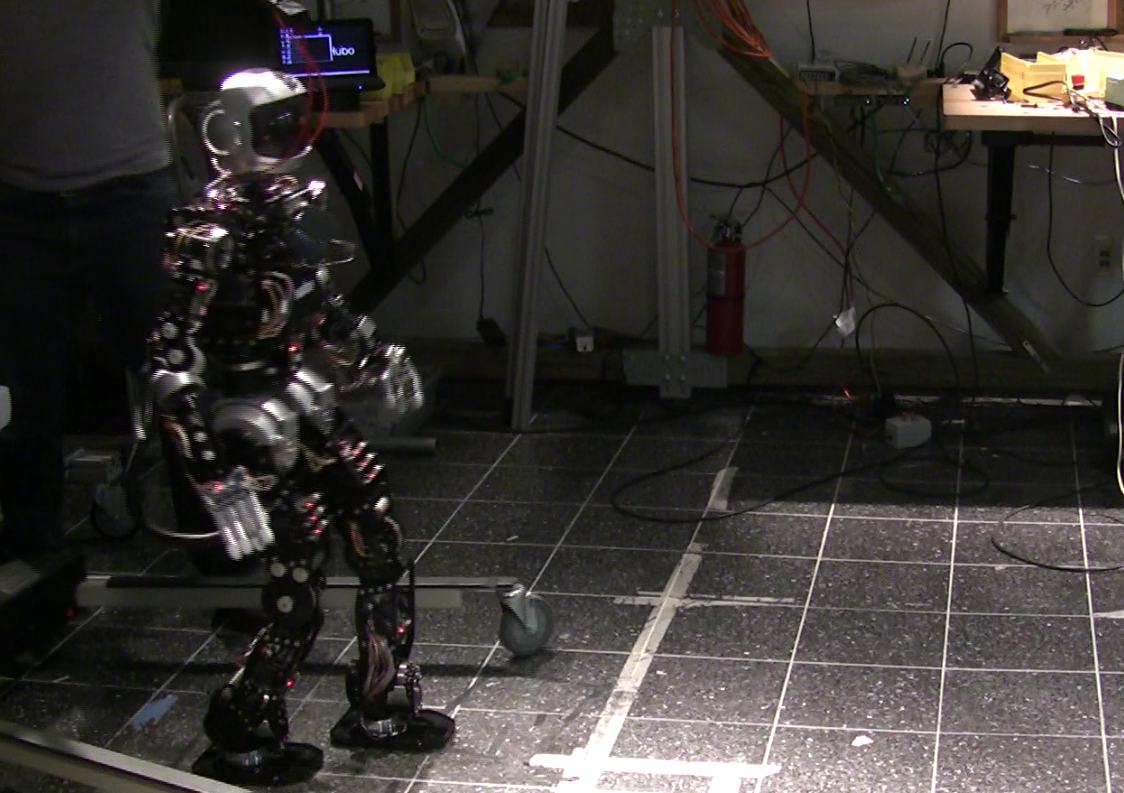
\includegraphics[width=0.6\columnwidth]{./examples/pix/hubo-walking.png}

\includegraphics[width=0.3\columnwidth]{./qrcode/qrcode-hubo-walking.png}\\
      Video: http://danlofaro.com/phd/walking/\#WalkingHubo
  \caption{Hubo2+ preforming ZMP walking using Hubo-Ach in real-time based on the walking pattern generated in Section~\ref{sec:WalkingPatternGeneration}.}
  \label{fig:RealHuboWalkingVideo}
\end{figure}

\begin{figure}[thpb]
  \centering
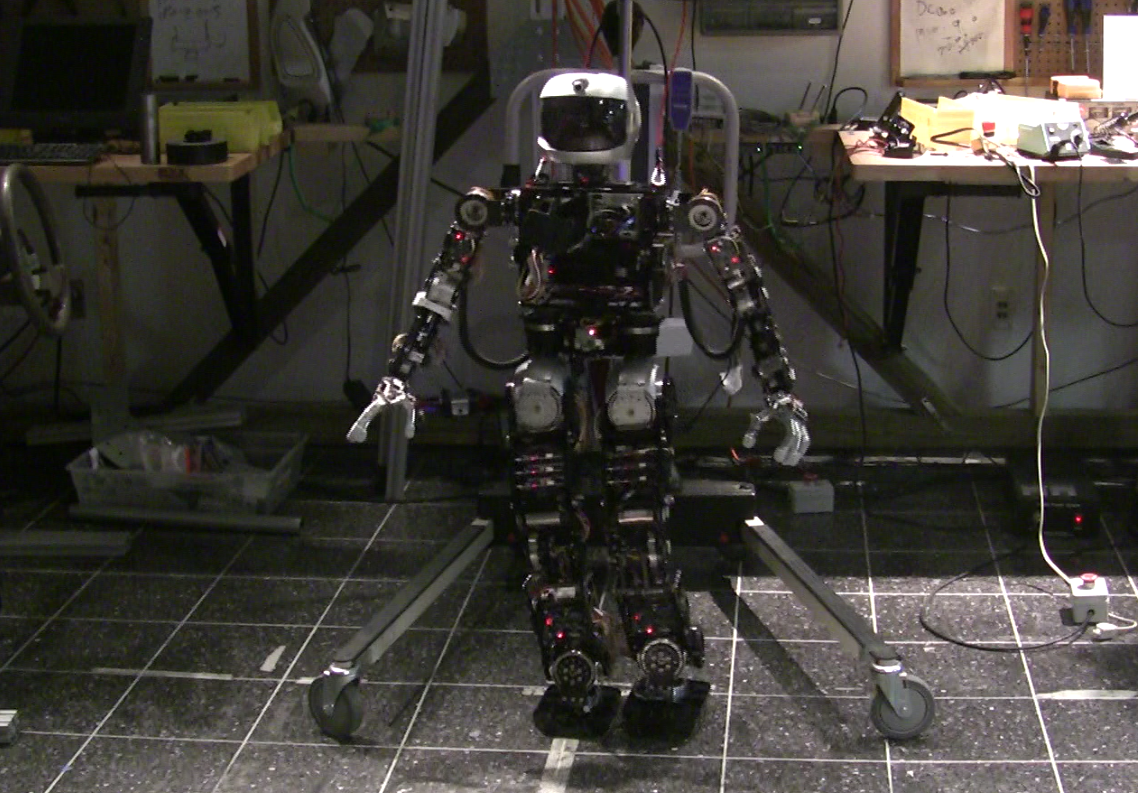
\includegraphics[width=0.6\columnwidth]{./examples/pix/hubo-walkinginplace.png}

\includegraphics[width=0.3\columnwidth]{./qrcode/qrcode-hubo-walkinginplace.png}\\
      Video: http://danlofaro.com/phd/walking/\#WalkingInPlaceHubo
  \caption{Hubo2+ preforming ZMP walking in place using Hubo-Ach in real-time based on the walking pattern generated in Section~\ref{sec:WalkingPatternGeneration} with a forward velocity of $0.0~\frac{m}{sec}$}
  \label{fig:RealHuboWalkingInPlaceVideo}
\end{figure}





%% ---------------- Hubo Walking in 5 days ------------------------
\subsection{Hubo Dynamic Walking - Developed in 5 Days Using Hubo-Ach}\label{sec:dynamicWalking}
Fig.~\ref{fig:dynamicwalking} shows Hubo2+ dynamic walking using Hubo-Ach as the primary controller.  The standard ZMP walking algorithms were implemented by our partners Mike Sillman and Matt Zucker at Geortia Gech and Swarthmore respectively.  All control was implemented using Daniel M. Lofaro's Hubo-Ach system.

\begin{figure}[thpb]
  \centering
  %\begin{tikzpicture}
    %\clip [rounded corners=1em] (0,0) rectangle coordinate (centerpoint) (5,7.5cm);
%    \node[minimum width=\linewidth,minimum height=174pt,draw=black,rounded corners=1em,fill=bgcolor,draw=black]
%    {};
%    \node[name=img] {
      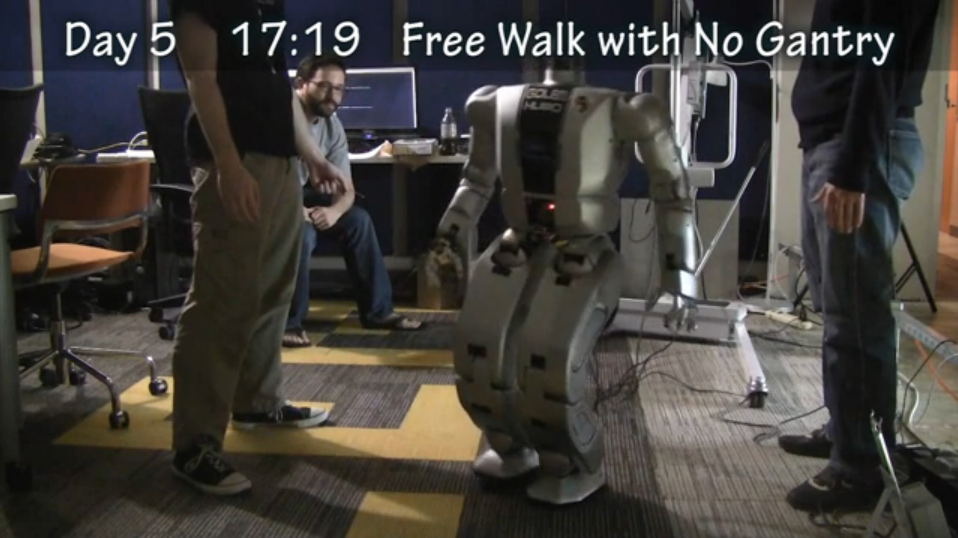
\includegraphics[width=0.6\columnwidth]{./examples/pix/dynamicwalking.png}
      
\includegraphics[width=0.3\columnwidth]{./qrcode/qrcode-dynamicwalking.png}\\
      Video: http://danlofaro.com/phd/walking/\#Walking5Days
%    };
%    \draw [bgcolor, rounded corners=1em, line width=1em,inner sep=0pt]
%    (img.north west) --
%    (img.north east) --
%    (img.south east) --
%    (img.south west) -- cycle
%    ;
%  \end{tikzpicture}
\caption{Hubo dynamic walking using Hubo-Ach as the primary controller.  The standard ZMP walking algorithms were implemented by our partners Mike Sillman and Matt Zucker at Geortia Gech and Swarthmore respectively.  All control was implemented using Daniel M. Lofaro's Hubo-Ach system.}
  \label{fig:dynamicwalking}
\end{figure}














%% Advanced Examples: Maybe add the title :advanced examples or somethign like that			
\section{Visual Serving Example}\label{sec:visuralServoing}
This section uses visual feedback using an RGB-D (Red Green Blue - Depth) camera and the walking trajectories given in Section~\ref{sec:walking:example}.
The goal of this experiment is to have the robot visually track an object, walk towards the object, and stop when it is within $0.2~m$ of it.

	\subsection{Tracking Using Vision}\label{sec:visTracking}
		Using a simple HSV (Hue Saturation Value) 

	\subsection{Visual servoing during full-body locomotion task}
		Hubo using Hubo-Ach to walk and track a blue box.  
The robot will walk towards the blue box until it is within $0.2~m$ at which point it will stop.  
If the box moves, the robot will turn to track the box.
It is tracking the box in work-space via an RGBD camera and the HSV tracking method discribed in Section~\ref{sec:visTracking}.
Section~\ref{sec:walking:example} discribes the method used for the walking task.
Fig.~\ref{fig:visualSeroving} shows the robot completing this task.

\begin{figure}[thpb]
  \centering
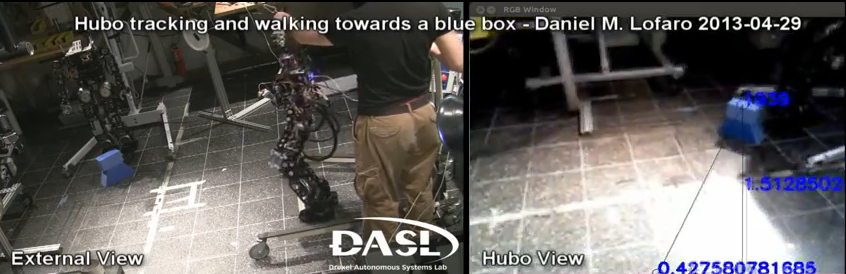
\includegraphics[width=0.79\columnwidth]{./pix/servoing.png}

\includegraphics[width=0.2\columnwidth]{./qrcode/qrcode-visualServoing.png}\\
     http://danlofaro.com/phd/tracking/\#TrackingAndWalking
  \caption{Hubo using Hubo-Ach to walk and track a blue box.  The robot will walk towards the blue box until it is within $0.2~m$ at which point it will stop.  If the box moves, the robot will turn to track the box.}
  \label{fig:visualSeroving}
\end{figure}

		


\section{Active Damping}\label{sec:activedamping}
	Using feedback from the force-torque sensors the Hubo-Ach controller adds compliance to the legs via active damping.
Fig.~\ref{fig:activedamping} shows as the user pushes down on the robot the force is detected by the force-torque (FT) sensors.
This then modifies the joint commands such that the center of mass (CoM) acts like there is an over-damped spring-damper system between it and mechanical ground.

\begin{figure}[thpb]
  \centering
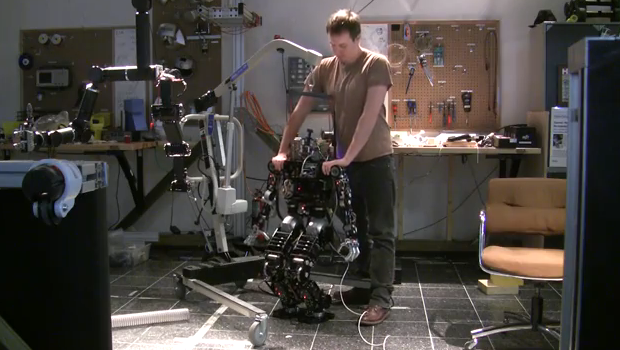
\includegraphics[width=0.6\columnwidth]{./pix/activedamping.png}

\includegraphics[width=0.3\columnwidth]{./qrcode/qrcode-activedamping.png}\\
     http://danlofaro.com/phd/activedamping/
  \caption{Using feedback from the force-torque sensors the Hubo-Ach controller adds compliance to the legs via active damping. }
  \label{fig:activedamping}
\end{figure}


%% One hubo then the other hubo moving example













